% !TeX spellcheck = en_US

% Summary // Introduction of the model

I develop a two-period OLG model that link age structure to labor share dynamics. I consider two types of households: young and old. The former are workers and the latter own the capital in the economy. This economy is closed and capital fully depreciates between two periods. Households determine public policy through probabilistic voting. The public policy and more specifically labor market institutions impact wage bargaining between the representative firm and the representative union. Bargaining also affects the desired public policy. Both jointly determine the state of the economy and therefore the labor share.

Households determine the public policy through a voting system maximizing their expected utility. While at the same time, the representative labor union bargains over wages with the representative firm. Both processes are independent and simultaneous. Thus, I assume that there is no coordination between households and the labor union. Indeed, the outcome of the voting process is determined by an aggregation of the individual households preferences. They cannot synchronize their vote with the representative union, neither the opposite. Therefore, the agents who operate within the wage bargaining take the voting outcome as given and vice versa.

\subsection{Households}\label{subsec:households}

The demographic dynamic of young households is $N^y_t = n_t N^y_{t-1}$ with $n_t > 0$ the gross young population growth. While the demographic dynamic of old households is $N^o_t = p_t N^y_{t-1}$ with $p_t \in \left(0,1\right]$ the survival rate.\footnote{The survival rate $p_t$ is an increasing function of the life expectancy and a decreasing function of the retirement age. In the model, agents are considered as old once they retire. If the life expectancy and the retirement age grow at the same rate, then the survival rate remains constant. For more details on the measurement of population aging, see \cite{Sanderson2007}; \cite{Sanderson2013}; \cite{DAlbis2013}.} Both demographic parameters follow deterministic processes. Thus, the old-age dependency ratio is $N^o_t/N^y_t = p_t/n_t$. The whole population is therefore $N_t = N^y_t + N^o_t$.

Each cohort consists of a continuum of homogeneous agents. Young households in period $t$ supply labor inelastically, earn a net income, consume and save for retirement. They face an idiosyncratic longevity risk: with probability $p_{t+1}$ they survive to become old households in period $t+1$. Once old, they pay taxes on their saving returns, consume and derive utility from government health spending. Finally, old households die at the end of the period. Savings of young agents who die before reaching old age are distributed among their surviving peers, reflecting a perfect annuities market.

Households derive utility from consumption when young $c_{1,t}$ and old $c_{2,t+1}$. Once old, they also value government health expenditure $h_{t+1}$. Agents discount the future at factor $\alpha \in \left(0,1\right)$. Due to risk of death, the effective discount factor of young households equals $\alpha p_{t+1}$.\footnote{Since the expected survival rate $p_{t+1}$ is an increasing function of the expected life expectancy. The longer an agent expects to live, the less they discounts future.} I assume that period utility functions are logarithmic. In first period, they earn a net income $y_t$ to allocate between consumption and savings $s_t$. In second period, they consume the net return of their savings $(1-\tau_{t+1}) s_t \hat{R}_{t+1}$, where $\tau_{t+1}$ is the tax rate and $\hat{R}_{t+1}$ the gross return on savings of a young household that survives to old age\footnote{Due to perfect annuity market $\hat{R}_t = R_t/p_t$ where $R_t$ is the gross return on physical capital.}. Maximizing expected utility, a household in period $t$ solves the following maximization problem:
	\begin{align*}
		\max_{\lbrace c_{1,t}, c_{2,t+1} \rbrace \geq 0} &\ln(c_{1,t}) + \alpha p_{t+1}\left\lbrace \ln(c_{2,t+1}) + \beta \ln(h_{t+1}) \right\rbrace\\
		\text{s.t.} ~~ & \begin{cases}
		c_{1,t} + s_t = y_t \\
		c_{2,t+1} = (1-\tau_{t+1}) s_t \hat{R}_{t+1}
		\end{cases}
	\end{align*}
where $\beta>0$ characterizes the preference for health expenditure. Solving the household maximization problem, I obtain the optimal consumption in both period and savings in first period for a household of type $i \in \lbrace e, u \rbrace$:
	\begin{align*}
		c^i_{1,t} &= \frac{1}{1+\alpha p_{t+1}} y^i_{t} \\
		c^i_{2,t+1} &= \frac{\alpha p_{t+1}}{1+\alpha p_{t+1}}(1-\tau_{t+1})\hat{R}_{t+1}y^i_{t} \\
		s^i_t &= \frac{\alpha p_{t+1}}{1+\alpha p_{t+1}} y^i_t
	\end{align*}
Since the utility function is logarithmic, this is a standard result where the saving is a constant proportion of the income.
Each household faces an idiosyncratic unemployment risk with probability $u_t \in \left[0,1\right)$. The income of an employed young agent is $y^e_t = (1-\tau_t)w_t$, while an unemployed young agent earns $y^u_t = b_t$, where $w_t$ is the wage and $b_t$ the unemployment benefits per capita. The aggregate saving in the economy is $S_t = (1-u_t) N_t^y s^e_t + u_t N_t^y s^u_t$. Thus,
	\begin{equation}\label{eq:agg_saving}
		S_t = \frac{\alpha p_{t+1}}{1+\alpha p_{t+1}}\left[ (1-u_t)(1-\tau_t)w_t + u_t b_t \right] N_t^y
	\end{equation}
The indirect utility of an old household at time $t$ depends on its income in $t-1$. Hence,
	\begin{equation}\label{eq:utility_old}
		U_t^{o,i} = \ln\left(\frac{\alpha p_t}{1+\alpha p_t}(1-\tau_t)y_{t-1}^i\hat{R}_t\right) + \beta \ln(h_t) ~~ \forall i = \lbrace e,u \rbrace
	\end{equation}
The indirect utility of a young household at time $t$ is:
	\begin{equation*}\label{eq:utility_young}
		U_t^{y,i} = \ln\left(\frac{1}{1+\alpha p_{t+1}}y_t^i\right)+ \alpha p_{t+1} U_{t+1}^{o,i} ~~ \forall i = \lbrace e,u \rbrace
	\end{equation*}
Computing the gap between employed and unemployed people in utility terms, I have:
	\begin{equation}\label{eq:utility_young_gap}
		U_t^{y,e} - U_t^{y,u} = (1+\alpha p_{t+1})\ln\left[\frac{(1-\tau_t)w_t}{b_t}\right]
	\end{equation}
Moreover, the expected income of each young household is a weighted average of both incomes (labor income and unemployment benefits). Thus, $\mathbb{E}(y_t) = (1-u_t)(1-\tau_t)w_t + u_tb_t$, where $\mathbb{E}$ is the expectation operator. Computing the expected utility of a young household at time $t$, I obtain:
	\begin{equation}\label{eq:expected_utility_young}
		\mathbb{E}({U}_t^y) = \ln\left(\frac{\mathbb{E}\left(y_t\right)}{1+\alpha p_{t+1}}\right) + \alpha p_{t+1}\left\lbrace \ln\left(\frac{\alpha p_{t+1}}{1+\alpha p_{t+1}}(1-\tau_{t+1})\mathbb{E}(y_t)\hat{R}_{t+1}\right) + \beta \ln(h_{t+1}) \right\rbrace
	\end{equation}

%% Production

\subsection{Production}

Firms are represented by a representative firm that uses a standard CES production function given by:
\begin{equation}\label{eq:prod}
Y_t = A\left[ \phi K_t^{\frac{\sigma - 1}{\sigma}} + (1-\phi) L_t^{\frac{\sigma - 1}{\sigma}}\right]^{\frac{\sigma}{\sigma-1}}
\end{equation}
where $K_t$ is the capital stock, $L_t$ the labor, $\sigma$ the elasticity of substitution between capital and labor, $\phi$ the factor share parameter allowing the relative importance of inputs in production to vary and $A$ a constant scale parameter. I do not consider any form of technical change, whether neutral or biased. Rewriting the production function in units of labor,
\begin{equation}\label{eq:prod/L}
\frac{Y_t}{L_t} = A\left(\phi k_t^{\frac{\sigma-1}{\sigma}} + 1-\phi\right)^{\frac{\sigma}{\sigma-1}}
\end{equation}
where $k_t\equiv K_t/L_t$ is the capital-per-worker (i.e. capital intensity). Since the economy is closed and capital fully depreciates between two periods, the capital in the economy is determined by the saving of the previous period, i.e. $K_t = S_{t-1}$. The labor-demand equation obtained from the profit maximization of the representative firm is:
\begin{equation}\label{eq:labor_demand}
w_t = (1-\phi)A\left(\phi k_t^{\frac{\sigma-1}{\sigma}}+1-\phi\right)^{\frac{1}{\sigma-1}}
\end{equation}
The labor demand elasticity is defined as $\mathcal{E}^{L,w}_t=\frac{\partial L_t}{\partial w_t}\frac{w_t}{L_t}$. Using the equation \eqref{eq:labor_demand},
\begin{equation}\label{eq:labor_elasticity}
\mathcal{E}^{L,w}_t = -\sigma\left(1+\frac{1-\phi}{\phi}k_t^{\frac{1-\sigma}{\sigma}}\right)
\end{equation}
Using equations \eqref{eq:prod/L} and \eqref{eq:labor_demand}, I compute the labor share $\theta_t = \frac{w_tL_t}{Y_t}$ which is:
\begin{equation}\label{eq:theta}
\theta_t = \left(1+\frac{\phi}{1-\phi}k_t^{\frac{\sigma-1}{\sigma}}\right)^{-1}
\end{equation}
This equation holds if and only if the representative firm is on its labor demand curve. Notice that when the capital-labor elasticity of substitution equals unity, then $\theta_t=1-\phi$. In this case, the production function is Cobb-Douglas and the labor income share is constant in $k_t$.  When $\sigma \to 0$, the production function is Leontief. When $\sigma \to +\infty$, the production function is linear. 
%\textbf{Yet, I do not consider these cases in the rest of the paper.} Hence, I define the elasticity of substitution between capital and labor such as $\sigma\in\mathbb{R}_+^\star\setminus\lbrace1\rbrace$. 
As long as the representative firm is not constrained in its ability to hire and fire workers, it means that the firm is on its labor demand curve and thereby the labor share only depends on $k_t$.\footnote{Considering a small open economy (SOE), the capital-labor ratio becomes constant. \cite{Schmidt2013} show that, in such a case, the labor share dynamics only reflects variations in net foreign assets of the economy.}

The comparative are straightforward,
\begin{equation*}
	\left\lbrace ~~
	\frac{\partial w_t}{\partial k_t} > 0,~~
	\frac{\partial (Y_t/L_t)}{\partial k_t} > 0,~~
	\frac{\partial \theta_t}{\partial k_t} \lessgtr 0 ~~
	\right\rbrace, ~~ \sigma \gtrless 1
\end{equation*}
A higher capital-labor ratio increases the wage resulting from the labor demand equation and the production-per-worker. However, the impact on the labor share depends on the elasticity of substitution between both input factors. When capital and labor are gross substitute (i.e. $\sigma > 1$), a higher capital-labor ratio decreases the labor share. While the relationship is positive when both input factors are gross complement (i.e. $\sigma < 1$). Since the labor share can be defined as the ratio between wage and production-per-worker, it means that with gross substitute input factors, a rise of the capital-per-worker increases more the production-per-worker relatively to the wage rate. Vice versa when $\sigma <1$. Thus,
\begin{equation*}
	\left\lbrace ~~
	\frac{\partial w_t}{\partial k_t} ~\lessgtr~ \frac{\partial (Y_t/L_t)}{\partial k_t} ~~
	\right\rbrace, ~~ \sigma \gtrless 1
\end{equation*}
In order to have a negative relationship between the capital-to-labor ratio and the labor share without the presence of biased technical change, both input factors must be gross substitute (i.e. $\sigma >1$).

\subsection{Public policy preferences}\label{subsec:public_policy_preferences}

The government taxes the labor income of young households and the savings return of old households in period $t$ at rate $\tau_t$. The government revenue is shared between unemployment benefits and health expenditure. Thus, the government budget constraint is the following: $\tau_t\left( w_t(1-u_t)N^y_t + R_t S_{t-1} \right) = b_t u_t N^y_t + h_t N^o_t$. Capital fully depreciates between two periods, thus  $R_t = r_t$ and $K_t = S_{t-1}$, where $r_t$ is the rental price of capital. Therefore, the government budget constraint can be written as follows:
\begin{equation} \label{eq:government_bc}
	\tau_t Y_t = b_t u_t N^y_t + h_t N^o_t
\end{equation}
Young and old agents have different objectives. Young households desire more unemployment benefits since they cover the risk to be unemployed. While the elderly desire more health spending because they derive utility from it. \textit{Everything else equal}, both desire less taxes as it reduces their disposable income. I modelize the age-related conflict in public policy with this trade-off but it could be extended to other public policy instruments. The central point is to oppose young and old households with different returns in utility terms of policy instruments.

\cite{Sorensen2013} analyzes cross-section survey data for 22 countries and shows that agents change their public spending preferences over their life-cycle. Thus, he provides evidence for an age-related selfishness in public spending preferences. However, this effect tends to be small and heterogeneous across countries. He argues that a gerontocracy is not very likely. In line with these results, I consider a probabilistic voting setup in contrast to the median voter setup. This latter setup would create two extreme regimes with one of them being a gerontocracy. It would also generate large changes in public policy if the median-voter switches from young to old or vice versa. Under probabilistic voting, the equilibrium policy platform is a continuous function of the old-age dependency ratio. This setup smooths public policy changes in line with the literature of recent politico-economic models.

With probabilistic voting, all agents vote for a policy platform $g_t = (\tau_t, b_t, h_t)$ represented by opportunistic candidates (or parties). Candidates try to maximize their probability to win the election. They differ in their popularity and there is an idiosyncratic bias among voters for one candidate or the others. Candidates know about these biases. At the equilibrium, all candidates choose the same policy platform $g_t^\star$ that maximize the political objective function $W_t(g_t)$.\footnote{See \cite{Lindbeck1987} for more details on the probabilistic-voting setup.}

This function depends on population share of each voter groups and their respective sensitivity of voting behavior to policy changes $\omega^i$. There are three groups of voter: young households; and old households who are divided in two subgroups according to their employment situation during the previous period because they did not earn the same income when they were young. Henceforth, they do not have the same saving returns and differ in their indirect utility (i.e. $U_t^{o,u}$ and $U_t^{o,e}$ given by \eqref{eq:utility_old}). However, I assume that all the elderly have the same sensitivity $\omega^o = \omega^{o,u} = \omega^{o,e}$. Thus, the equilibrium public policy solves the following maximization program:
\begin{align*}
	\max_{g_t} ~ W_t(g_t) &= \frac{N_t^y}{N_t} \omega^y \mathbb{E}\left[U_t^y(g_t)\right] + \frac{N_t^o}{N_t} \omega^o \Big\{ u_{t-1} U_t^{o,u}(g_t) + (1-u_{t-1}) U_t^{o,e}(g_t) \Big\} \\
	\text{s.t.} ~~ & \eqref{eq:utility_old}, \eqref{eq:expected_utility_young}, \eqref{eq:government_bc}
\end{align*}
I assume that households only care about direct effects of public policy on their utility. They do not consider indirect effects of public policy on their utility that would pass through economic variables.\footnote{An interpretation of this assumption is that agents are not able to predict what will be the response of the labor market to changes in public policy. Otherwise stated, the investment of effort to be perfectly informed and able to calculate indirect effects of different public policies is too costly for an individual (or at least a representative share of the electorate). Thus, the rationality is limited to direct effects on the utility function. This is related to political science literature and the concept of \textit{synoptic rationality}. See \cite{Meier1980} for more details.} Let $\tilde{U}^i_t$ be the part of the utility which is directly affected by the public policy platform. From \eqref{eq:utility_old}, it is straightforward that $\tilde{U}_t^o = \tilde{U}_t^{o,u} = \tilde{U}_t^{o,e}$. Therefore, the political objective function can be rewritten as:
\begin{equation*}
	W_t(g_t) = \frac{N_t^o}{N_t} \omega^o \tilde{U}_t^o(g_t) + \frac{N_t^y}{N_t} \omega^y \tilde{U}_t^y(g_t) + \dots
\end{equation*}
where $\dots$ denotes all the terms that are not directly affected by the public policy. Let $\omega$ be the \textit{relative ideological spread-out} of the elderly with respect to the youth. This relative ideological spread-out is characterized by the ratio of the sensitivities of voting behavior to policy changes for each group. Thus, $\omega \equiv \omega^o/\omega^y$. I assume that this spread-out is constant over time.\footnote{Two interpretation are plausible for this assumption: either both relative ideological spread-outs are time invariant; or they vary in same proportions. An interesting point would be to endogenize these spread-outs or to make them cohort-specific. Nevertheless, this goes beyond the scope of this paper.} Using equations \eqref{eq:utility_old} and \eqref{eq:expected_utility_young}, I rewrite the maximization program that characterize the public policy equilibrium as:
\begin{align*}
	\max_{\lbrace\tau_t, b_t, h_t\rbrace\geq 0} W_t(\tau_t, b_t, h_t) &= \ln(1-\tau_t) +\beta \ln(h_t) + \eta_t \ln\left[(1-u_t)(1-\tau_t)w_t + u_t b_t\right] + \dots \\
	\text{s.t.} ~~ &\tau_t Y_t = b_t u_t N^y_t + h_t N^o_t
\end{align*}
where $\eta_t = \frac{n_t}{p_t}\frac{1+\alpha p_{t+1}}{\omega}$ is the youth political weight. This variable is the channel through which the age structure affects the public policy. It depends negatively on the old-age dependency ratio $p_t/n_t$, the older the population the lower the political weight of the youth within the policy determination. It also depends negatively on the relative ideological spread-out $\omega$. The less ideological is the youth, the higher will be its political weight. If young people are less ideologically tenacious, then they are easier to convince with an appropriated public policy. As a consequence, candidates pay more attention to them.\footnote{Otherwise stated, the less spread-out is the ideology distribution within a group, the more numerous to swing are the voters after changes in public policy platform.} $\eta_t$ is increasing in $\alpha p_{t+1}$ corresponding to the fact that young voters are more likely to swing in favor of a pro-labor-income policy platform. Because the longer they expect to live, the more they will have to save in order to smooth their consumption. Therefore, they require a relatively greater income which can only be a labor one.

Focusing on the interior solution, first order conditions lead to the following public policy preferences:
%The first-order conditions with respect to $\tau_t$, $b_t$ and $h_t$, are respectively:
%\begin{align*}
%	\frac{1}{1-\tau_t} + \frac{\eta_t(1-u_t)w_t}{(1-u_t)(1-\tau_t)w_t + u_t b_t} &= \lambda \frac{Y_t}{N_t^y} + \mu_\tau\\
%	\frac{\eta_t u_t}{(1-u_t)(1-\tau_t)w_t + u_t b_t} &= \lambda u_t +\mu_b \\
%	\frac{\beta}{h_t} &= \lambda \frac{p_t}{n_t} + \mu_h
%\end{align*}
%where $\lambda$ is the Lagrangian multiplier and $\mu_j ~~\forall j = \lbrace \tau, b, h\rbrace$ denotes the multiplier associated with the non-negativity constraint on the policy instrument $j$. Focusing on the interior solution (i.e. $\mu_\tau = \mu_b = \mu_h = 0$) and manipulating the previous first-order conditions, I obtain the public policy preferences :
\begin{align}
	\frac{b_t}{(1-\tau_t)w_t} &= \frac{1-u_t}{u_t} \left(\eta_t\frac{1-\theta_t}{\theta_t}- 1\right)
	\label{eq:inverse_replacement_rate}\\
	\tau_t &= 1 - \left[\left(1-\theta_t\right)\left(1+\beta+\eta_t\right)\right]^{-1}
	\label{eq:tax_rate} \\
	h_t N^o_t &= \frac{\beta}{1+\beta+\eta_t}Y_t
	\label{eq:health_expenditure}
\end{align}
%% Comparative statics of public policy %%
Where the first equation is the unemployment replacement rate, the second the tax rate and the third the government health expenditure. Some comparative statics about previous results are straightforward,
\begin{equation*}
	\left\lbrace \frac{\partial \frac{b_t}{(1-\tau_t)w_t}}{\partial \eta_t} > 0, ~ \frac{\partial \tau_t}{\partial \eta_t} > 0, ~\frac{\partial h_t}{\partial \eta_t} < 0\right\rbrace
\end{equation*}
Young generations desire more redistribution and a higher unemployment replacement rate because they face an unemployment risk. Such a public policy allows them to increase their expected income. However, they vote to reduce the government health spending because they do not derive utility from it yet.\footnote{I do not consider any form of explicit altruism. However, the parameter $\beta$ which is the preference for government health spending captures a form of altruism from young to their elders. The greater the parameter, the more individuals care about government health spending once old. Finally, a form of explicit altruism from young to old generations would smooth the results and soften the age-related conflict.}

The aggregated income of young households is $Y_t^y = \left[(1-u_t)(1-\tau_t)w_t+b_tu_t\right]N_t^y$. Using equation \eqref{eq:inverse_replacement_rate} and \eqref{eq:tax_rate}, it can be written as a share of the total income $Y_t$ such that:
\begin{equation*}
Y_t^y = \frac{\eta_t}{1+\beta+\eta_t} Y_t
\end{equation*}
%Young households decide to save a share of their income in order to smooth their consumption for the second period, this share depends on their life expectancy. The remaining income is consumed. From section \ref{subsec:households}, these shares are:
%\begin{align*}
%S_t = \frac{\alpha p_{t+1}}{1+\alpha p_{t+1}} Y_t^y \\
%C_{1t} = \frac{1}{1+\alpha p_{t+1}} Y_t^y
%\end{align*}
The government health spending for old households is given by equation \eqref{eq:health_expenditure}. The total income is split between incomes of both groups and the government health spending. Thus, $Y_t = Y_t^y + Y_t^o + h_tN_t^o$. Hence, the remaining part of the total income is the aggregated income of the elderly:
\begin{equation*}
Y_t^o = \frac{1}{1+\beta+\eta_t} Y_t
\end{equation*}
For a given level of total income $Y_t$, the comparative statics are unambiguous. When the youth political weight raises ($\eta_t \nearrow$), young households increase their aggregated income with more redistribution (i.e. $\frac{\partial Y_t^y}{\partial \eta_t}>0$). Conversely, the aggregated income of the elderly decreases (i.e. $\frac{\partial Y_t^o}{\partial \eta_t}<0$) and so does the government health spending (i.e. $\frac{\partial(h_tN_t^o)}{\partial \eta_t}<0$). Such a raise may be due to two reasons: either a decrease of the old-age dependency ratio ($p_t/n_t \searrow$) or an increase of the survival rate of the current young generation ($p_{t+1} \nearrow$). The first reason is directly related to the old-age related conflict within the public policy. However, the second reason open onto an important point of the aging population. $p_{t+1}$ can be interpreted as the expected life expectancy. Expecting to live longer, agents save more in order to smooth their consumption for the second period.\footnote{See, for example, \cite{Bloom2003}; \cite{Zhang2005}.} From equation \eqref{eq:agg_saving}, the saving share of the aggregated income of young households is increasing in life expectancy. Therefore, a longer expected life expectancy leads to more savings and thus more available capital for the next period. Furthermore, it is possible to express the after-tax income ratio between young and old households as:
\begin{equation} \label{eq:after_tax_income_ratio}
	\frac{Y_t^y}{Y_t^o} = \eta_t
\end{equation}
As expected, the greater is the political weight of the youth, the greater is the redistribution and so is the gap between both incomes.
% Transition
These public policy instruments interact with the outcome of the wage bargaining to determine the state of the economy.

\subsection{Wage bargaining}\label{subsec:wage_bargaining}
There is a single union that represents the workers. In order to modeling the wage bargaining, I consider a ``Right-to-manage'' model \textit{à la} \cite{Nickell1983}. The union bargains only over wages with the employer retaining the prerogative to hire and fire.\footnote{Another possibility would have been to consider an ``Efficient contract'' model \textit{à la} \cite{McDonald1981} where the union bargains over wages and employment. However, this specification does not correspond to the data as \cite{Bentolila2003} showed. Moreover, it would add a lot of complexity to the model without a substantial gain in the analysis.} Consequently, the firm is always on its labor demand curve and equation \eqref{eq:labor_demand} holds. The union wants to maximize the workers' utility compared to the unemployed people's one (i.e. $U^{y,e}_t - U^{y,u}_t$) as described by \eqref{eq:utility_young_gap}. The representative firm maximizes its outside option which is $Y_t-w_tL_t$ corresponding to $r_t K_t$. Thus, the outcome of the bargaining process is determined by the maximization program as follows:
\begin{align*}
\max_{w_t>0} ~~ &\lbrace \left(L_t[U^{y,e}_t - U^{y,u}_t]\right)^\gamma \left(Y_t-w_tL_t\right)^{1-\gamma}\rbrace\\
\text{s.t.} ~~ &U_t^{y,e} - U_t^{y,u} = (1+\alpha p_{t+1})\ln\left[\frac{(1-\tau_t)w_t}{b_t}\right]
\end{align*}
where $\gamma\in(0,1)$ is the relative bargaining power of the union. The first-order condition can be expressed as:
\begin{equation*}\label{eq:foc_wage_bargaining}
\frac{\gamma}{1-\gamma}\left\lbrace\mathcal{E}^{L,w}_t\ln\left[\frac{(1-\tau_t)w_t}{b_t}\right]+1\right\rbrace = \ln\left[\frac{(1-\tau_t)w_t}{b_t}\right] \frac{w_tL_t}{Y_t-w_tL_t}
\end{equation*}
where $\mathcal{E}^{L,w}_t$ is the labor demand elasticity. Using the equations \eqref{eq:labor_elasticity} and \eqref{eq:theta} within the first-order condition of the wage bargaining, I can express the capital-per-worker as a function of the unemployment replacement rate:
\begin{equation}\label{eq:k(x)}
k_t(X_t) = \left[\frac{1-\phi}{\phi}\frac{1-\gamma(1-\sigma)}{\gamma}\frac{X_t}{1-\sigma X_t}\right]^{\frac{\sigma}{\sigma-1}}
\end{equation}
where $X_t=\ln\left[\frac{(1-\tau_t)w_t}{b_t}\right]$ is the value-added to be employed in utility terms which only depends on the unemployment replacement rate. Since the capital-per-worker has to be positive, it implies that $1-\sigma X_t > 0$. The maximum capital-labor elasticity of substitution ensuring that this condition is met can be defined as the function $\bar{\sigma}(x) = -\log^{-1}(x)$, where $x$ is the unemployment replacement rate. Figure \ref{fig:xsigma} plots this function for all values of the unemployment replacement rate between 0 and 0.8. The minimum unemployment replacement rates for France and the United-States over the period 1970-2010 correspond, respectively, to 0.592 and 0.567. Hence, the condition is met for all $\sigma$ between zero and $1.907$ for France or $1.762$ for the United-States. For the remaining part of the paper, I assume that $\frac{1}{X_t}>\sigma$ is always satisfied.

\begin{figure}[tb]
	\centering
	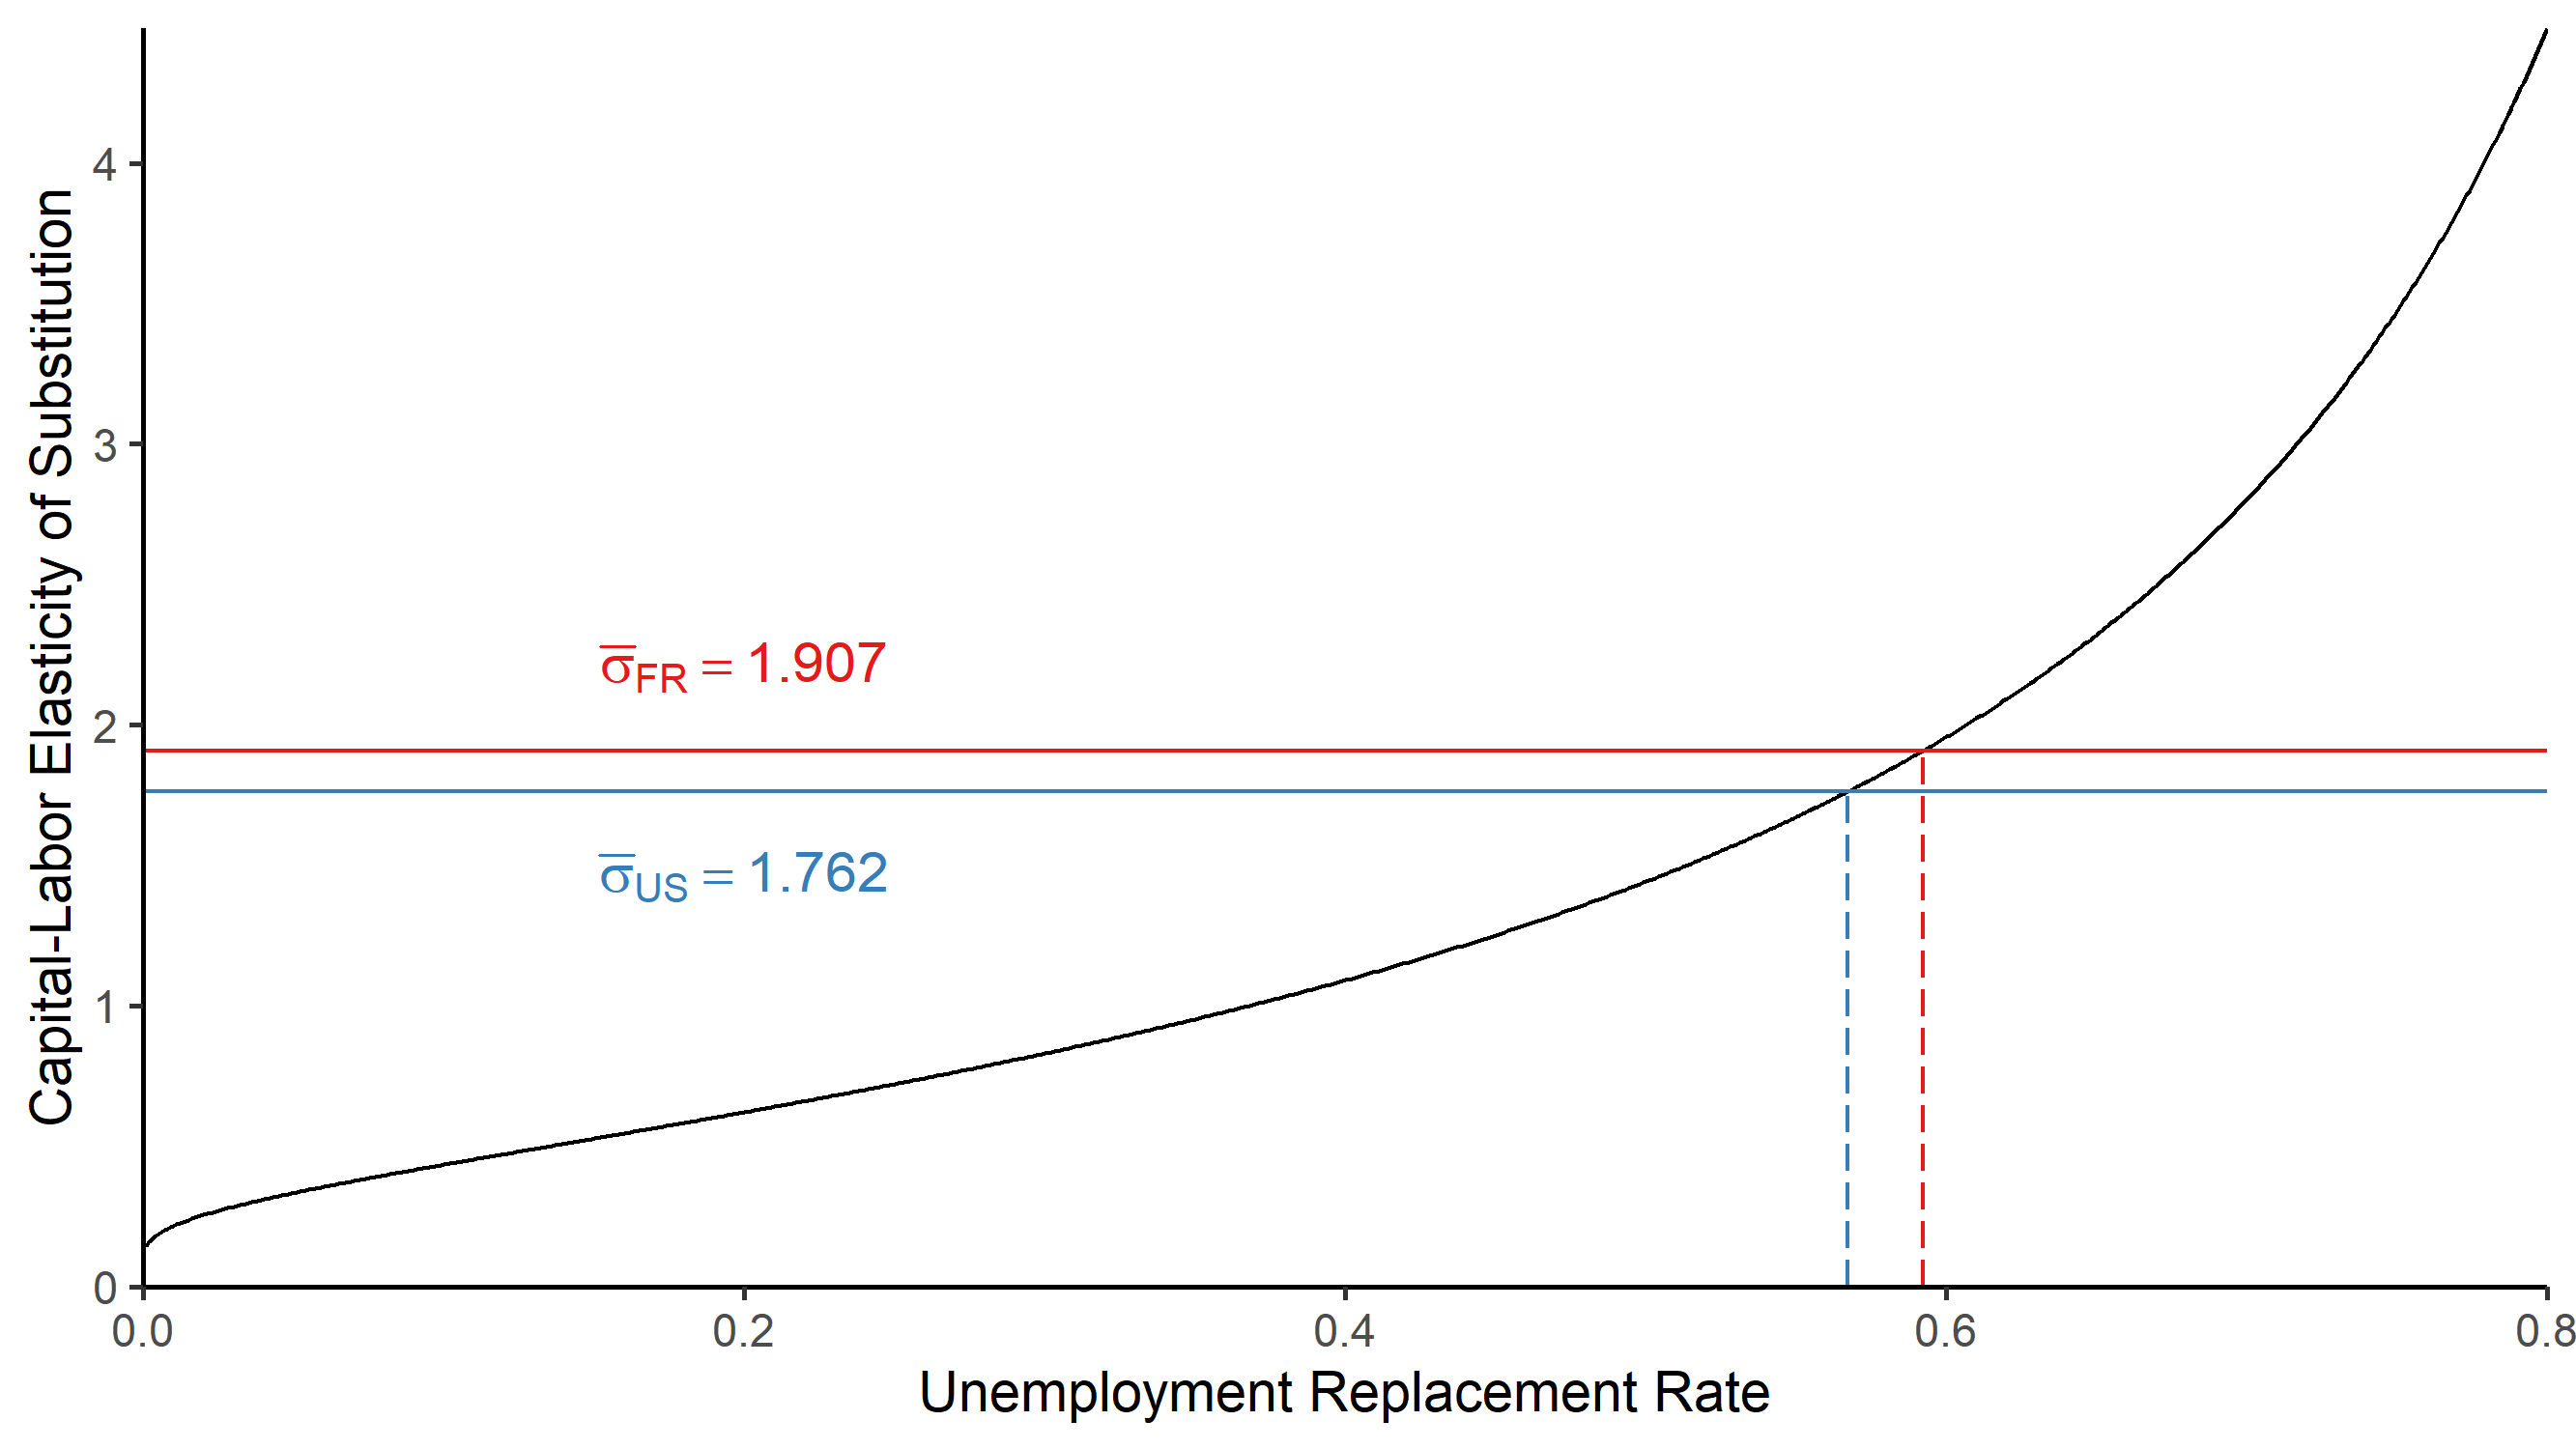
\includegraphics[width = 1\linewidth]{../result/xsigma.png}
	\caption{Maximum capital-labor elasticity of substitution ($\bar{\sigma}$) for France (red) and the United-States (blue).}
	\label{fig:xsigma}
	\vspace{.5ex}
	\hrule
	\vspace{-4ex}
	\justify\singlespacing\footnotesize Unemployment replacement rate data are from the \href{http://cwed2.org/}{Comparative Welfare Entitlements Dataset 2 (CWED 2)}, see \cite{CWED2017} for more details.
\end{figure}
% The greater is the unemployment replacement rate, the smaller is the value-added to have a job (i.e. $X_t$).
%All comparative statics are derived in \textbf{Appendix}.
Comparative statics with respect to $X_t$ are the following:
\begin{equation*}
\left\lbrace \frac{\partial k_t}{\partial X_t} \gtrless 0 \Rightarrow 
\left\lbrace \frac{\partial w_t}{\partial X_t} \gtrless 0,~~
\frac{\partial (Y_t/L_t)}{\partial X_t} \gtrless 0,~~ \frac{\partial w_t}{\partial X_t} <
\frac{\partial (Y_t/L_t)}{\partial X_t} \right\rbrace \Rightarrow 
\frac{\partial \theta_t}{\partial X_t} < 0
\right\rbrace, ~~ \sigma \gtrless 1
\end{equation*}
When the unemployment replacement rate increases ($\frac{b_t}{(1-\tau_t)w_t} \nearrow$), it decreases the value-added to have a job ($X_t \searrow$). Hence, the labor share increases ($\theta_t \nearrow$). As an interpretation, when the unemployment replacement rate increases it allows the union to bargain a higher wage and so to grab a relatively larger share of the income. This mechanism holds whatever the value of the capital-labor elasticity of substitution (i.e. $\sigma$). This is an interesting result in the sense that usually CES production functions give rise to results with a threshold on the value of $\sigma$ with respect to unity. However, intermediate partial derivatives are just transitional and consider only the partial effect of a change in the unemployment replacement rate. Due to the endogeneity of $w_t$, I save the mechanisms analysis for later. 

% Let us focus on the case where capital and labor are gross substitute (i.e. $\sigma>1$). The higher is the unemployment replacement rate, the stronger is the outside option of the representative union which increases the bargained wage with the firm. When the capital and labor are gross substitute (i.e. $\sigma>1$), the firm will compensate the increase in wage by using more capital than labor. Since the representative firm is always on its labor demand curve, \textit{other things equal}, it reduces the labor demand and therefore labor input. Reducing the labor input does shrink the production level of the representative firm. As a result, the labor income share decreases.

\subsection{Equilibrium}\label{equilibrium}

Voting and wage bargaining take place simultaneously and there is no-coordination between both of them. As a consequence, both processes take the outcome of the other as given. The interaction determines the state of the economy. Expressing equations \eqref{eq:inverse_replacement_rate} and \eqref{eq:k(x)} in the value of being employed $X_t$ as a function of the capital-to-labor ratio. The capital-to-labor ratio $k_t$ at the equilibrium solves:
\begin{align}
	\label{eq:Xg} 
	X_t &= \ln\left( \frac{ \frac{N_t^y}{K_t} k_t - 1 } { \frac{\phi}{1-\phi} k_t^{\frac{\sigma-1}{\sigma}} \eta_t - 1 }\right) \\
	\label{eq:Xh}
	X_t &= \left( \sigma + \frac{1-\phi}{\phi} \frac{1-\gamma(1-\sigma)}{\gamma} k_t^{\frac{1-\sigma}{\sigma}} \right)^{-1} 
\end{align}
The Cobb-Douglas case (i.e. $\sigma = 1$) can be solved analytically and leads to the following equilibrium:
\begin{align*}
	X_t &= \frac{\gamma}{1-\phi(1-\gamma)} \\
	k_t &= \left[1 + e^{X_t}\left(\frac{\phi}{1-\phi}\eta_t-1\right)\right]\frac{K_t}{N_t^y}
\end{align*}
The value-added to have a job $X_t$ is constant. The capital-per-worker $k_t$ is still determined by demographic variables and is proportional to the capital-per-young individual. However, this case is not really useful to determine labor share's dynamics. Because the labor share becomes constant over time from equation \eqref{eq:theta}, i.e. $\theta_t = 1-\phi$. Otherwise, there is uniqueness of the equilibrium for any other value of sigma. Proof in \hyperref[appendix:uniqueness]{appendix A}. The equilibrium is characterized by 13 equations:
\begin{align}
\eta_t &= \frac{n_t}{p_t}\frac{1+\alpha p_{t+1}}{\omega} \tag{Pub. $\eta$} \\
X_t &= \ln\left( \frac{ \frac{N_t^y}{K_t} k_t - 1 } { \frac{\phi}{1-\phi} k_t^{\frac{\sigma-1}{\sigma}} \eta_t - 1 }\right) \tag{Eq. $g$} \\
X_t &= \left( \sigma + \frac{1-\phi}{\phi} \frac{1-\gamma(1-\sigma)}{\gamma} k_t^{\frac{1-\sigma}{\sigma}} \right)^{-1} \tag{Eq. h}\\
L_t &= \frac{K_t}{k_t} \tag{Prod. $L$} \\
w_t &= A(1-\phi)\left( \phi k_t^\frac{\sigma-1}{\sigma} + 1-\phi \right)^\frac{1}{\sigma-1} \tag{Prod. $w$}\\
Y_t &= A \left[ \phi K_t^\frac{\sigma-1}{\sigma} + (1-\phi) L_t^\frac{\sigma-1}{\sigma} \right]^\frac{\sigma}{\sigma-1} \tag{Prod. $Y$}\\
u_t &= 1 - \frac{L_t}{N_t^y} \tag{Prod. $u$}\\
\theta_t &= \left(1 + \frac{\phi}{1-\phi} k_t^\frac{\sigma-1}{\sigma} \right)^{-1} \tag{Prod. $\theta$} \\
\tau_t &= 1 - \left[ (1-\theta_t)(1+\beta+\eta_t) \right]^{-1} \tag{Pub. $\tau$}\\
b_t &= (1-\tau_t) w_t e^{-X_t} \tag{Pub. $b$}\\
h_t &= \frac{\tau_t Y_t - b_t u_t N_t^y}{N_t^o} \tag{Pub. $h$}\\
S_t &= \frac{\alpha p_{t+1}}{1 + \alpha p_{t+1}} \left[ (1-\tau_t)w_t(1-u_t) + b_tu_t \right] N_t^y \tag{HH. $S$}  \\
K_{t+1} &= S_t	\tag{HH. $K$}
\end{align}
Let define, respectively, equations \eqref{eq:Xg} and \eqref{eq:Xh} with the functions $g(L_t, K_t, \eta_t, N_t^y; \phi, \sigma)$ and $h(L_t, K_t; \sigma, \phi, \gamma)$, such as:
\begin{align*}
	X_t &= g(L_t, K_t, \eta_t, N_t^y; \phi, \sigma) 
	%&= \ln\left[ \frac{ \frac{N_t^y}{L_t} - 1 } { \frac{\phi}{1-\phi} \left(\frac{K_t}{L_t}\right)^{\frac{\sigma-1}{\sigma}} \eta_t - 1 }\right]
	\\
	X_t &= h(L_t, K_t; \sigma, \phi, \gamma) 
	%&= \left[ \sigma + \frac{1-\phi}{\phi} \frac{1-\gamma(1-\sigma)}{\gamma} \left(\frac{K_t}{L_t}\right)^{\frac{1-\sigma}{\sigma}} \right]^{-1}
\end{align*}
Differentiating this system,
\begin{align*}
	dX_t &= g_L dL_t + g_K dK_t + g_\eta d\eta_t + g_{N^y} dN_t^y \\
	dX_t &= h_L dL_t + h_K dK_t
\end{align*}
where $f_x$ is the partial derivative of the $f$ function with respect to the variable $x$, e.g. $g_L = \frac{\partial g}{\partial L_t}$. Solving the system,
\begin{equation*}
	dL_t = \frac{1}{h_L-g_L}\left[(g_K-h_K) dK_t + g_\eta d\eta_t + g_{N^y} dN_t^y \right]
\end{equation*}
The variables $\eta_t$ and $N_t^y$ are given by demographic dynamics. The capital stock $K_t$ is given by the savings of the previous period. Thus, the variable that determines the equilibrium is the level of employment $L_t$. Partial derivatives are derived in \hyperref[appendix:derivatives]{appendix B}. $g_\eta$ is negative because the greater is the youth political power, the greater are the unemployment benefits and so the smaller is the value-added to have a job in utility terms. $g_{N^y}$ is positive because the more numerous are the young individuals, the more these unemployment benefits are divided among them and so the smaller is the value-added to have a job in utility terms. $g_K-h_K$ depends on the value of $\sigma$ with respect to unity, i.e. $g_K-h_K \lessgtr 0, ~ \forall \sigma \gtrless 1$. This is directly related to the fact that both input factors are either gross substitute or gross complement. When labor and capital are gross substitute, more available capital stock requires less labor for a given of level of output. Otherwise, when both are complement, the representative firm has to jointly increase labor with capital stock in order to maintain the same production level. Finally, the sign of $h_L-g_L$ is ambiguous regardless of the value of $\sigma$. When $\sigma < 1$, then $g_L$ and $h_L$ are both positive. Thus, $g_L-h_L$ is ambiguous. When $\sigma > 1$, $h_L$ is unambiguously negative. But the sign of $g_L$ cannot be determined without additional assumptions. If $\frac{\eta_t}{\Theta_t} > \sigma$, then $g_L$ is negative. Otherwise, $g_L$ is negative if the unemployment rate is lower than a certain threshold, i.e $u_t < \bar{u}_t$ where $\bar{u}_t = \left(2 - \frac{\eta_t}{\Theta_t\sigma}\right)^{-1}$. Thus, when the unemployment rate is high enough such that $u_t > u_t^\star$, $g_L$ is unambiguously positive and so is $g_L-h_L$. This is the only case where it is possible to determine unambiguously the impact of variables on $L_t$. In such a case, $\frac{dL_t}{dK_t}\Bigr|{\substack{d\eta_t = 0\\dN_t^y = 0}} < 0$, $\frac{dL_t}{dN^y_t}\Bigr|{\substack{dK_t = 0\\d\eta_t = 0}} > 0$ and $\frac{dL_t}{d\eta_t}\Bigr|{\substack{dK_t = 0\\dN_t^y = 0}} < 0$. Therefore, expect in this special case, $g_L-h_L$ is also ambiguous. Due to the indeterminacy of $g_L$, I perform a quantitative analysis in section \ref{sec:quantitative_analysis}.


